\raggedright
\section{Introduzione}
\subsection{Descrizione generale e funzionamento}
\par Questo progetto ha l'obiettivo di sviluppare un modulo hardware programmabile in linguaggio VHDL per leggere e processare una sequenza di dati memorizzati in celle alterne della memoria.
\par Il modulo inizia l'elaborazione quando riceve un segnale di avvio e un indirizzo iniziale.
  La sequenza da processare ha una lunghezza specificata.
  Il modulo legge i dati dalla memoria e sostituisce ogni valore nullo con l'ultimo valore valido letto. Inoltre, calcola un indicatore di "credibilità" per ciascun valore, da inserire nella cella adiacente: questo indicatore inizia da 31 per ogni valore diverso da zero e diminuisce ogni volta che si incontra un valore nullo, senza mai scendere sotto zero.
  Se il primo valore della sequenza è nullo, esso rimane tale e il valore di credibilità associato viene impostato a zero. Lo stesso accade fino al raggiungimento del primo valore valido.
\par L'elaborazione termina quando il modulo ha finito di aggiornare la sequenza e i relativi valori di credibilità, segnalando la fine del processo con un segnale di completamento. Il modulo si resetta e si prepara per una nuova esecuzione del processo.
\subsection{Interfaccia del componente}
  Di seguito vengono riportati i segnali che consentono la comunicazione tra la memoria ed il componente progettato.
\begin{itemize}
  \item \textbf{{i\_clk}:} sincronizza le operazioni del componente.
  \item \textbf{{i\_rst:}} inizializza il componente per ricevere il primo segnale di START.
  \item \textbf{{i\_start}:} avvia l'elaborazione dei dati.
  \item \textbf{{i\_k}:} rappresenta la lunghezza della sequenza di dati.
  \item \textbf{{i\_add}:} rappresenta l'indirizzo di memoria da cui iniziare l'elaborazione della sequenza.
  \item \textbf{{o\_done}:} indica al Test Bench la fine dell'elaborazione.
  \item \textbf{{o\_mem\_addr}:} contiene l'indirizzo di memoria al quale leggere/scrivere il dato.
  \item \textbf{{i\_mem\_data}:} contiene il dato letto all'indirizzo specificato.
  \item \textbf{{o\_mem\_data}:} contiene il dato da scrivere all'indirizzo specificato.
  \item \textbf{{o\_mem\_en}:} abilita la comunicazione con la memoria.
  \item \textbf{{o\_mem\_we}:} abilita la scrittura in memoria.
\end{itemize}
\begin{figure}[H]
  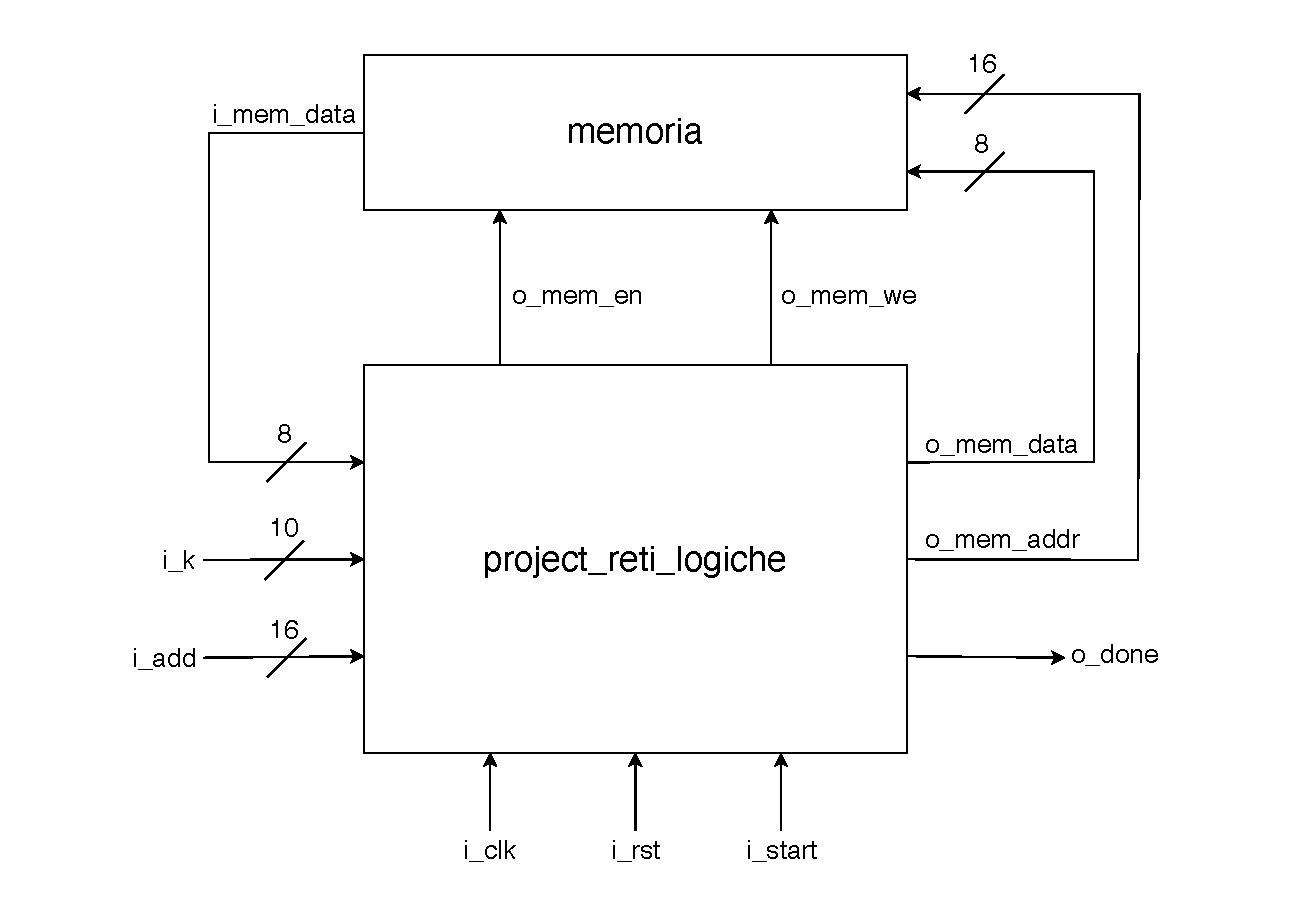
\includegraphics[width = 1\textwidth]{images/interfaccia_componente.pdf}
  \caption{Interfaccia del componente}
\end{figure}
\pagebreak

\section{Architettura}
  \par Per affrontare il problema, abbiamo adottato un approccio modulare, scomponendo il sistema in componenti distinti, ognuno dei quali è implementato come un processo separato nel codice VHDL del componente.
    Questa suddivisione consente di isolare e gestire singolarmente le diverse responsabilità funzionali del sistema, migliorando la leggibilità e la manutenibilità del codice.
    L'architettura complessiva comprende cinque moduli principali che collaborano per elaborare correttamente la sequenza di dati.
  \par L'approccio modulare è stato scelto per diversi motivi validi.
    In primo luogo, facilita la verifica e il debug del sistema, permettendo di testare e validare ciascun modulo in modo indipendente.
    In secondo luogo, promuove la riusabilità del codice, poiché moduli ben definiti possono essere riutilizzati in altri progetti o contesti.
    Infine, questa architettura consente una maggiore flessibilità e scalabilità, rendendo più semplice l'implementazione di modifiche o l'aggiunta di nuove funzionalità senza compromettere l'intero sistema.
  \begin{figure}[H]
  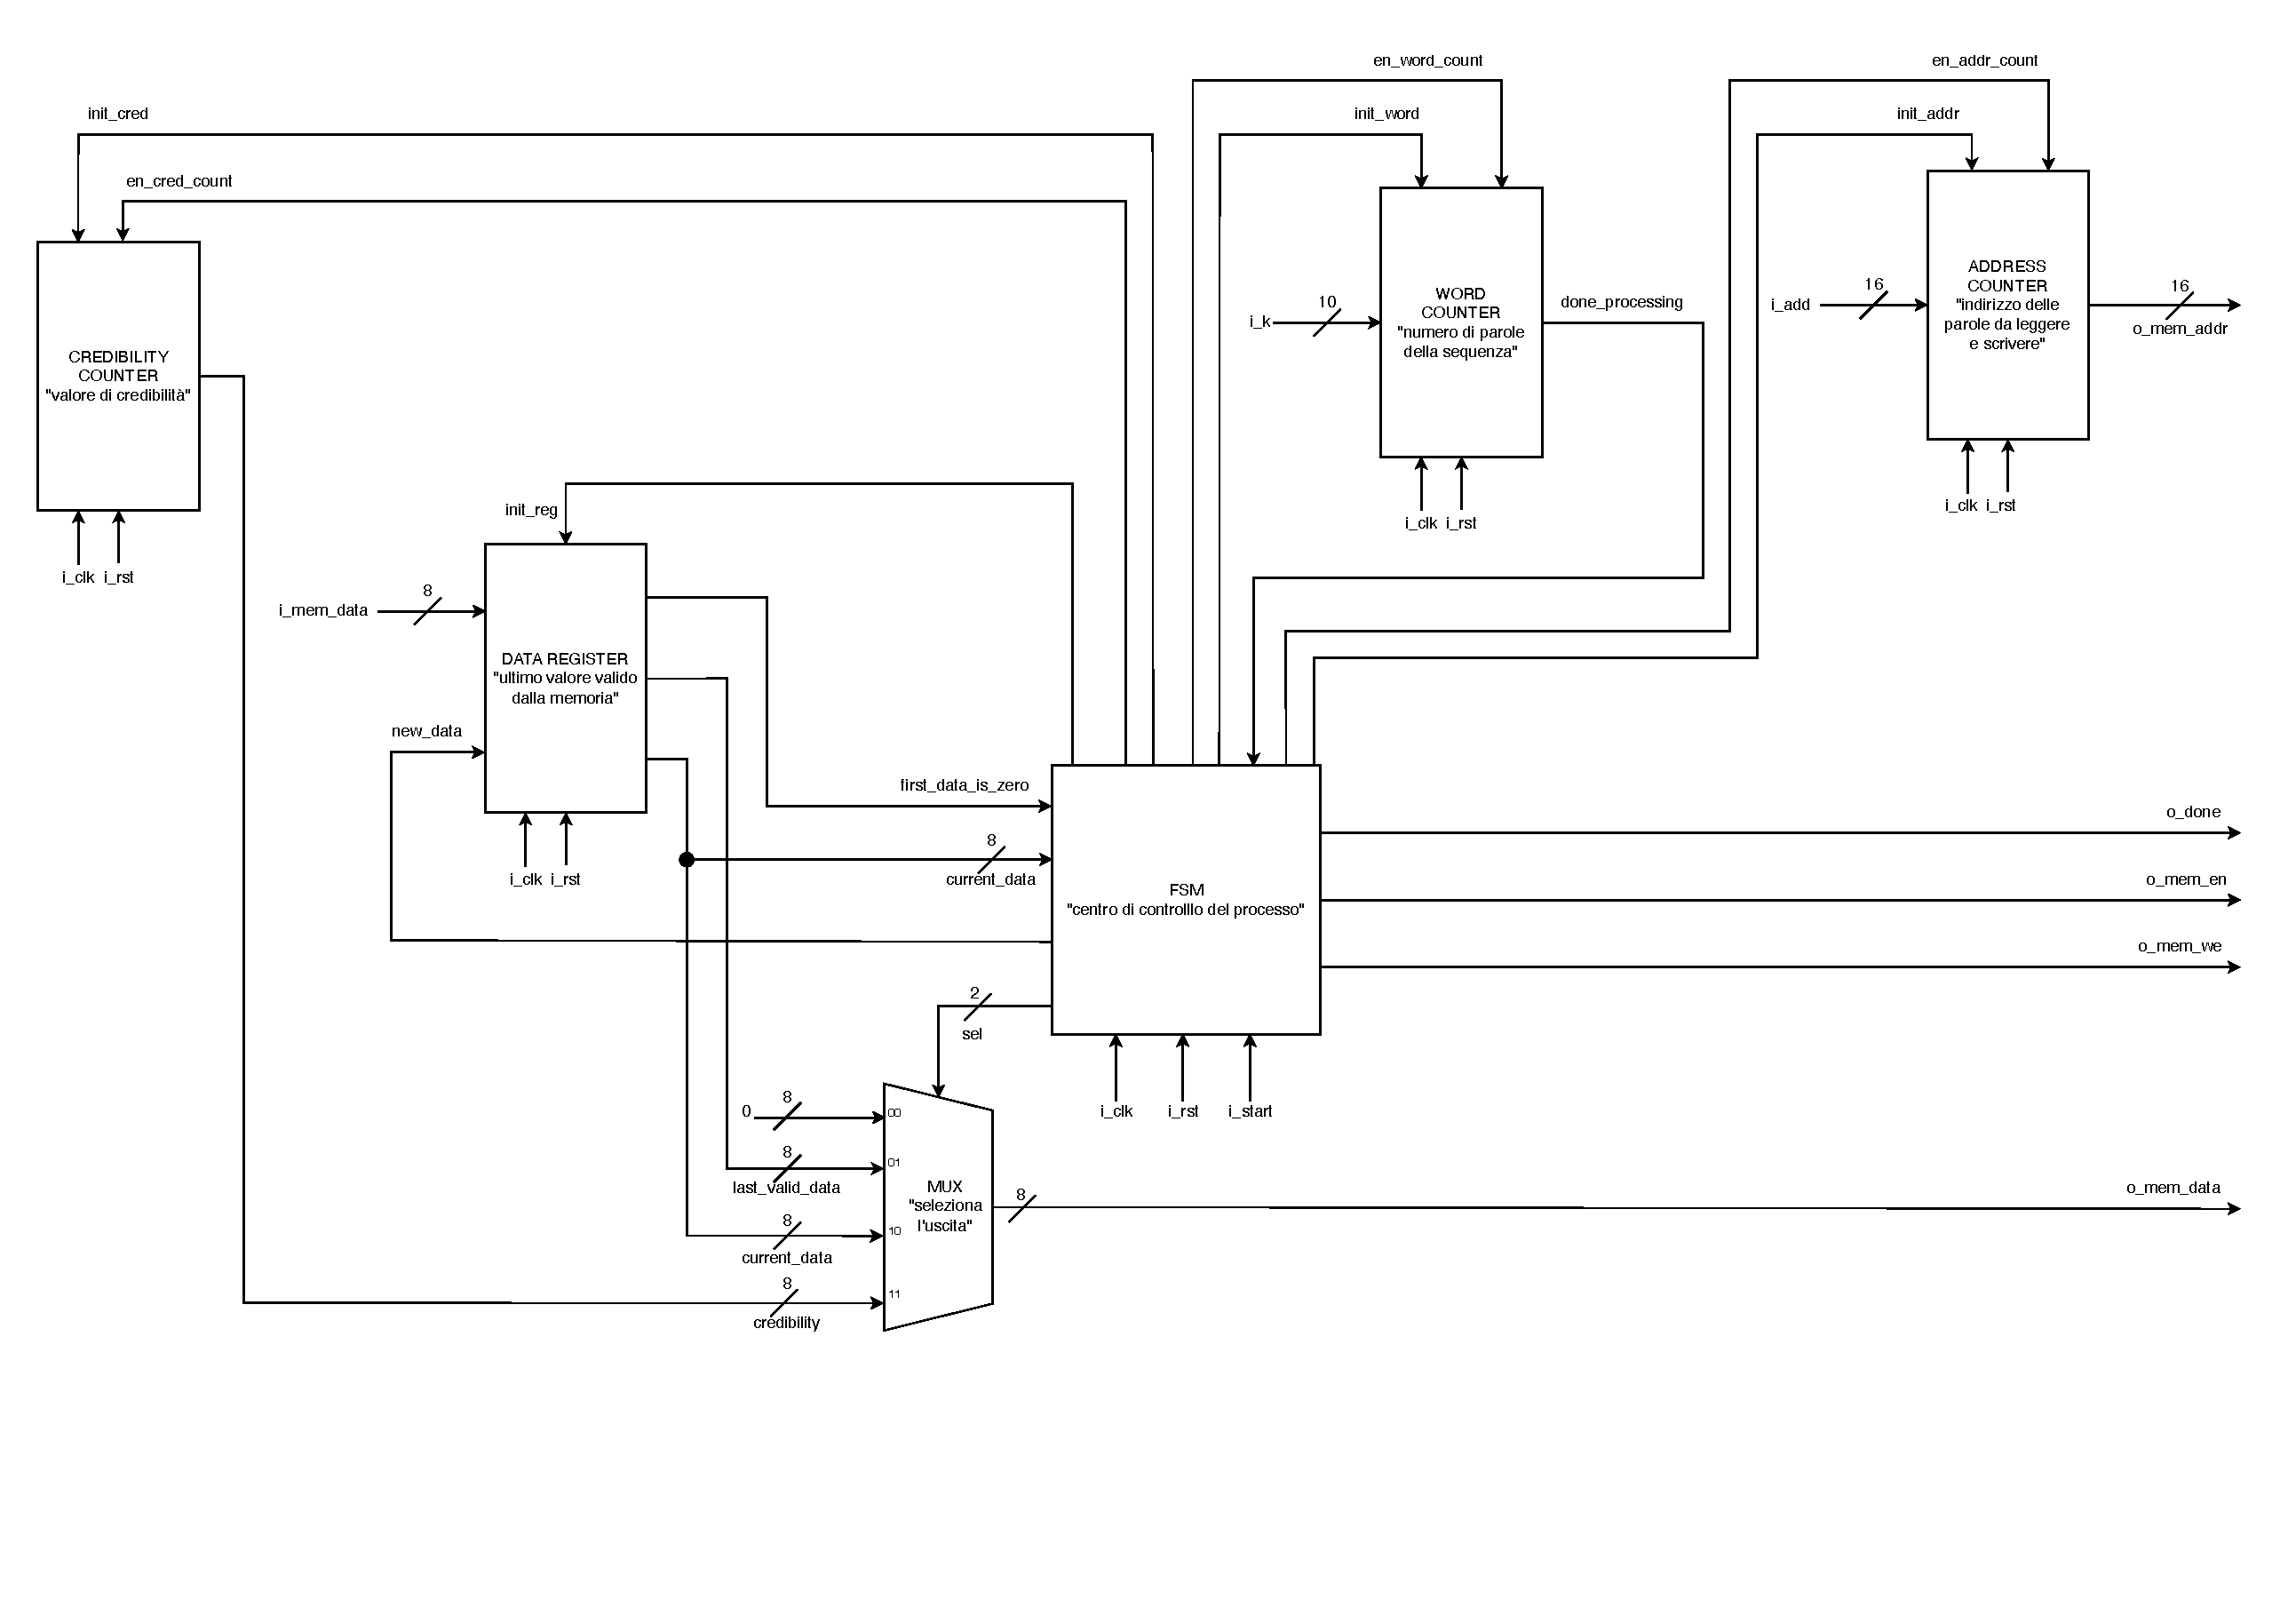
\includegraphics[width=1.1\textwidth, left]{images/schema_a_blocchi_compontente.pdf}
  \caption{Schema a blocchi del componente}
\end{figure}
\subsection{Segnali interni}
  Di seguito una breve descrizione di tutti i segnali interni utilizzati per implementare le funzionalità del componente.
\begin{itemize}
  \item \textbf{{first\_data\_is\_zero}:} flag utilizzato per la gestione del caso particolare in cui il primo valore è zero.
  \item \textbf{{curr\_addr}:} memorizza l'indirizzo corrente al quale leggere/scrivere i dati in memoria.
  \item \textbf{{credibility}:} rappresenta il valore di credibilità corrente.
  \item \textbf{{word\_count}:} rappresenta il numero di parole lette dalla memoria.
  \item \textbf{{en\_addr\_count}:} abilita il modulo che si occupa di calcolare il corretto indirizzo di memoria.
  \item \textbf{{en\_word\_count}:} abilita il modulo contatore di parole.
  \item \textbf{{en\_cred\_count}:} abilita il modulo che si occupa di calcolare il valore di credibilità per la parola corrente.
  \item \textbf{{init\_addr}:} reinizializza il modulo Address counter.
  \item \textbf{{init\_word}:} reinizializza il modulo Word counter.
  \item \textbf{{init\_cred}:} reinizializza il modulo Credibility counter.
  \item \textbf{{init\_reg}:} reinizializza il modulo Data register.
  \item \textbf{{sel}:} indica quale valore collegare all'uscita.
  \item \textbf{{last\_valid\_data}:} mantiene l'ultimo valore valido letto dalla memoria.
  \item \textbf{{current\_data}:} memorizza il valore corrente appena letto dalla memoria.
  \item \textbf{{new\_data}:} comunica che un nuovo valore valido è stato letto dalla memoria.
  \item \textbf{{done\_processing}:} comunica il termine della computazione.
\end{itemize}
\subsection{Moduli}
\subsubsection{Address counter}
 Calcola l'indirizzo della cella di memoria del dato da leggere o scrivere.
 Ad inizio computazione 'curr\_addr' viene posto uguale a 'i\_add'.
 Successivamente viene incrementato di un'unità sul fronte di salita del clock se il segnale di 'en\_addr\_count' è attivo, mentre in presenza di un segnale di reset 'curr\_addr' viene riportato a zero.
\subsubsection{Word counter}
 Conta fino al numero di parole $K$.
 Il conteggio parziale, inizialmente posto a zero, viene incrementato di un'unità ogni volta che viene letta una parola dalla memoria.
 Una volta raggiunto il valore $K$ fornito dal testbench, il segnale 'done\_processing' viene attivato, indicando la conclusione della computazione.
 In presenza di un segnale di reset sia 'word\_count' che 'done\_processing' vengono riportati a zero.
\subsubsection{Credibility counter}
 Calcola il valore di credibilità che viene scritto in memoria durante la computazione.
 Partendo dal valore $31$ di default, esso rimane tale se viene letta una parola diversa da zero, mentre viene decrementato di un'unità (senza mai scendere al di sotto di zero) per ogni dato non valido consecutivo letto.
 In presenza di un segnale di reset, 'credibility' torna al suo valore di default.
\subsubsection{Data register}
Aggiorna tutti i segnali associati alla lettura del dato corrente.
In particolare, ad ogni ciclo di clock, se non c'è stata nessuna reinizializzazione, il segnale `current\_data` viene aggiornato con il valore di `i\_mem\_data`.
Inoltre, se `new\_data` è uguale a 1, `first\_data\_is\_zero` viene impostato a zero e `last\_valid\_data` viene aggiornato con il valore di `i\_mem\_data`.
\subsubsection{Multiplexer}
 In base al valore del segnale di selezione, l'uscita 'o\_mem\_data' viene collegata al corrispondente dato da scrivere in memoria.
\subsubsection{Macchina a stati}
  \par L'ultimo componente del modulo progettato è la macchina a stati finiti, che ha il compito di gestire l'intero processo di elaborazione della sequenza in ingresso.
    La FSM coordina le operazioni degli altri componenti, assicurando che ogni fase dell'elaborazione avvenga nell'ordine corretto e nel momento opportuno.
  \par Di seguito vengono elencati gli stati della macchina con le relative uscite.
    Gli stati $S2$, $S3$ ed $S5$ sono considerati stati \textit{idle} e non producono alcuna uscita.
    Tuttavia, si è rivelato necessario aggiungerli in fase di progettazione per garantire la corretta sincronizzazione dei moduli tra loro e con il clock.
  \begin{itemize}
    \item \textbf{$S0$:} Questo è lo stato iniziale della FSM.
      La transizione verso S1 avviene quando il segnale `i\_rst` viene abbassato.
    \item \textbf{$S1$:} Stato di setup in cui tutti i moduli vengono reinizializzati, preparandoli per una nuova computazione non appena il segnale `i\_start` viene alzato.
      Viene abilitata la comunicazione con la memoria.
    \item \textbf{$S2$:} Stato di attesa dell'arrivo di una nuova parola, viene attraversato ciclicamente per scorrere l'intera sequenza di dati.
      Una volta che `done\_processing` viene alzato, avviene la transizione verso lo stato $S7$.
    \item \textbf{$S4$:} In questo stato, i segnali vengono gestiti in base al valore letto dalla memoria.
      Se il primo valore della sequenza è nullo, il segnale di selezione viene modificato per portare un valore nullo in uscita.
      Se invece è un valore nullo in mezzo alla sequenza, il segnale per attivare \textit{Credibility counter} viene alzato e la selezione cambia per portare in uscita l'ultimo valore valido letto.
      Se il valore letto è diverso da zero, \textit{Credibility counter} viene reinizializzato, il segnale `new\_data` viene alzato e la selezione viene modificata per portare in uscita il dato corrente.
      Indipendentemente dal valore letto, viene abilitata la scrittura in memoria e attivato \textit{Address counter}.
    \item \textbf{$S6$:} Stato che modifica la selezione per la scrittura della credibilità.
      Viene scritto 0 se non è mai stato letto un valore non nullo, altrimenti viene scritto il valore contenuto in \textit{Credibility}.
      Inoltre, i segnali per l'abilitazione della scrittura e dei moduli \textit{Address counter} e \textit{Word counter} vengono alzati.
    \item \textbf{$S7$:} Stato di attesa che aspetta che il segnale `i\_start` venga abbassato, permettendo così di tornare allo stato di setup $S1$.
  \end{itemize}

  \begin{figure}[H]
    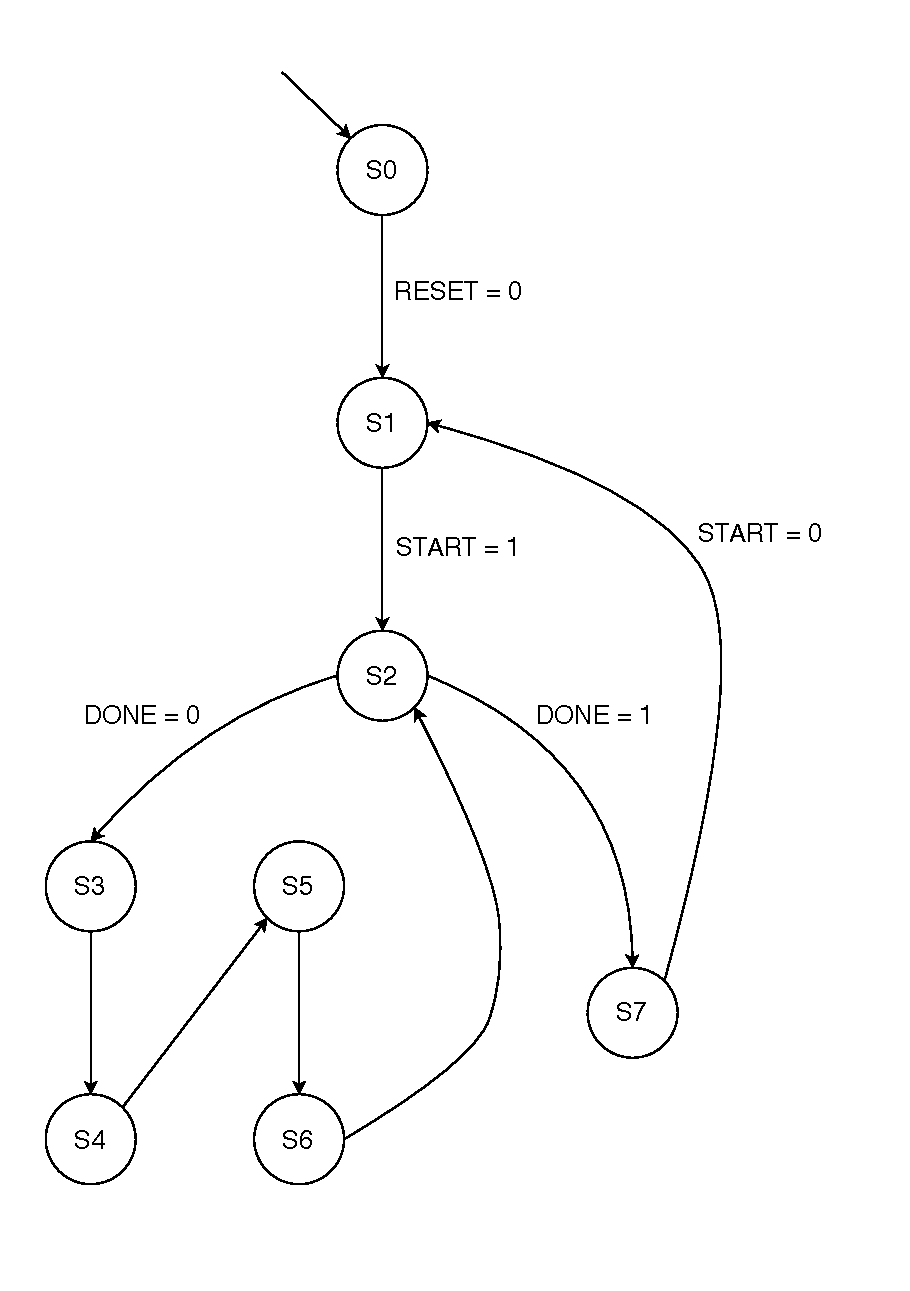
\includegraphics[width = .6\textwidth, center]{images/fsm_diagram.pdf}
    \caption{Macchina a stati finiti}
  \end{figure}
\pagebreak

\section{Risultati sperimentali}
\subsection{Sintesi}
\subsubsection{Report utilization}
\begin{verbatim}
    +-------------------------+------+-------+------------+-----------+-------+
    |        Site Type        | Used | Fixed | Prohibited | Available | Util% |
    +-------------------------+------+-------+------------+-----------+-------+
    | Slice LUTs*             |   63 |     0 |          0 |     78600 |  0.08 |
    |   LUT as Logic          |   63 |     0 |          0 |     78600 |  0.08 |
    |   LUT as Memory         |    0 |     0 |          0 |     26600 |  0.00 |
    | Slice Registers         |   57 |     0 |          0 |    157200 |  0.04 |
    |   Register as Flip Flop |   57 |     0 |          0 |    157200 |  0.04 |
    |   Register as Latch     |    0 |     0 |          0 |    157200 |  0.00 |
    | F7 Muxes                |    0 |     0 |          0 |     39300 |  0.00 |
    | F8 Muxes                |    0 |     0 |          0 |     19650 |  0.00 |
    +-------------------------+------+-------+------------+-----------+-------+
\end{verbatim}
\par Solo una minima parte delle \textit{Lookup Table} e dei registri disponibili sulla scheda $Artix-7 FPGA xc7a200tfbg484-1$ utilizzata in fase di sintesi è stata necessaria per implementare il componente progettato.
\par Inoltre, nessuno dei registri utilizzati è del tipo \textit{Latch}, condizione necessaria a garantire l'assenza di ritardi di propagazione indesiderati.
\subsubsection{Report timing}
\begin{verbatim}
Slack (MET) :       17.369ns  (required time - arrival time)
  Source:           current_data_reg[3]/C
                      (rising edge-triggered cell FDCE clocked by clock
                        {rise@0.000ns fall@5.000ns period=20.000ns})
  Destination:      credibility_reg[0]/CE
                      (rising edge-triggered cell FDPE clocked by clock
                        {rise@0.000ns fall@5.000ns period=20.000ns})
  Path Group:       clock
  Path Type:        Setup (Max at Slow Process Corner)
  Requirement:      20.000ns  (clock rise@20.000ns - clock rise@0.000ns)
  Data Path Delay:  2.210ns  (logic 0.540ns (24.434%)  route 1.670ns (75.566%))
  Logic Levels:     3  (LUT4=1 LUT5=1 LUT6=1)
\end{verbatim}
\par Il progetto deve funzionare con un periodo di clock di almeno 20 ns, e questo requisito è stato verificato e rispettato come mostrato nel report di timing fornito dall'ambiente di sviluppo. Il tempo di percorso dati (data path delay) è di soli 2.210 ns, suddiviso tra logica (0.540 ns) e routing (1.670 ns).
\par Questo ampio margine di slack conferma che il progetto è in grado di operare correttamente con il periodo di clock specificato, garantendo la stabilità e l'affidabilità del dispositivo anche nelle condizioni di processo più lente.
\subsection{Simulazioni}
  \par Abbiamo testato il comportamento del nostro dispositivo in vari casi limite, conformi e coerenti con le specifiche, che abbiamo ritenuto rilevanti per assicurarci del suo corretto funzionamento.
  \par Durante le simulazioni, abbiamo assunto che tutti i dati forniti dal test bench e dalla memoria fossero sempre nel formato desiderato e privi di errori fondamentali. Di conseguenza, non abbiamo implementato controlli aggiuntivi sugli input, concentrandoci invece sull'elaborazione e la gestione efficiente dei dati forniti.
\subsubsection{Sequenza vuota}
  Abbiamo verificato il comportamento del nostro dispositivo con una sequenza vuota, ossia una sequenza con lunghezza $K=0$.
  In questo scenario, il modulo dovrebbe immediatamente segnalare il completamento dell'elaborazione tramite il segnale $DONE$ senza effettuare alcuna operazione di lettura o scrittura in memoria.
  Questo test garantisce che il dispositivo gestisca correttamente il caso limite di una sequenza priva di dati, evitando operazioni inutili.
\subsubsection{Elaborazione multipla}
  Per testare la capacità del dispositivo di gestire più elaborazioni consecutive, abbiamo eseguito una serie di cicli di avvio ($START$) e completamento ($DONE$).
  Ogni ciclo ha comportato l'elaborazione di una nuova sequenza di dati con diverse lunghezze e indirizzi di partenza.
  Questo test ha confermato che il dispositivo può reinizializzarsi correttamente tra un'elaborazione e l'altra e che tutte le operazioni vengono eseguite senza errori o conflitti.
\subsubsection{Reset asincrono}
  Abbiamo introdotto il segnale di reset asincrono ($RESET$) durante diverse fasi dell'elaborazione per assicurare che il dispositivo si re-inizializzi correttamente.
  Questo test ha dimostrato che il modulo è in grado di interrompere l'elaborazione corrente e tornare allo stato iniziale in modo affidabile, privo di malfunzionamenti, e pronto per ricevere un nuovo segnale di $START$.
\subsubsection{Test completo}
  Il test completo ha coinvolto l'elaborazione di una sequenza di dati complessa, includendo diversi casi limite come la presenza di valori zero all'inizio, in mezzo e alla fine della sequenza.
  Abbiamo verificato che il modulo sostituisse correttamente i valori zero con l'ultimo valore valido e calcolasse i valori di credibilità in modo accurato.
  Questo test ha confermato il corretto funzionamento del dispositivo in un ambiente realistico e complesso, assicurandone la robustezza e l'affidabilità.
\pagebreak

\section{Conclusioni}
  \par Il progetto offre l'opportunità di sviluppare competenze nell'ambito della progettazione di hardware dedicato all'elaborazione e alla gestione efficiente dei dati.
  \par Attraverso questo lavoro, è stato possibile acquisire una più profonda comprensione delle metodologie e delle tecniche necessarie per implementare sistemi sincroni nel campo dell'ingegneria hardware.
  \par La capacità di tradurre concetti teorici in soluzioni pratiche e funzionali è un risultato significativo di questo lavoro, dimostrando la nostra preparazione nell'affrontare sfide complesse.
\pagebreak
